\documentclass{standalone}


\usepackage{tikz}
\usepackage{pgfplots}
\usepackage{tkz-euclide}

\pgfplotsset{compat=1.6}

\usetikzlibrary{positioning,calc}
\usetikzlibrary{arrows} 
\usetikzlibrary{patterns} 
\usetikzlibrary{shapes}
\usetikzlibrary{decorations.pathmorphing}

\begin{document}

\def\BeforeLight{2}
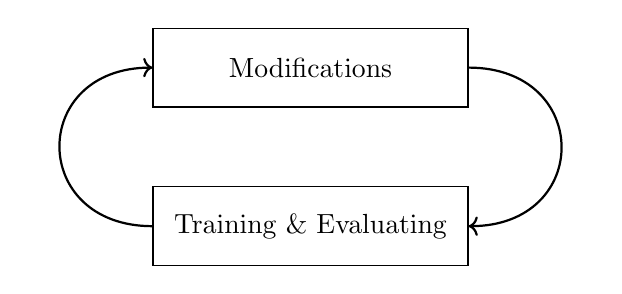
\begin{tikzpicture}
  % \draw[step=1cm, gray!20!white, very thin] (-5,-5) grid (5,5);

  \node[draw, minimum height=1cm,minimum width=4cm] at (0, 3) (mod)             {Modifications};
  \node[draw, minimum height=1cm,minimum width=4cm] (train) [below=1cm of mod] {Training \& Evaluating};

  \draw [->, thick] (mod.east) to [out = 0, in = 0, looseness = 2] (train.east);
  \draw [->, thick] (train.west) to [out = 180, in = 180, looseness = 2] (mod.west);

\end{tikzpicture}
\end{document}
